
\chapter{Experimentos e resultados}
% Label para referenciar
\label{experimentos-resultados}

% Diminuir espaçamento entre título e texto
\vspace{-1.9cm}

% Texto do capítulo

 Neste capítulo vamos abordar o ambiente de testes para os nossos protótipos, apresentar 
 o plano de testes utilizado e os resultados obtidos e análise dos dados.

\section{Ambiente de testes}
\label{ambientedetestes}

  Para efetuar os testes, os protótipos tiveram de ser colocados em um ambiente de testes. 
  Para os dois protótipos, hospedamos a aplicação em uma VPS da empresa Digital Ocean\footnote{Empresa Digital Ocean. Disponível em http://digitalocean.com}.
  Este servidor privado foi escolhido por ser o melhor custo beneficio para hospedagens de aplicações na Internet 
  devido ao seu baixo busto (5 dólares mensais). Comparando-o com outras empresas que oferecem serviços semalhante
  tais como Linode \footnote{Empresa Linode. Disponível em https://www.linode.com}, Rackspace \footnote{Empresa RackSpace. Disponível em http://www.rackspace.com/cloud/servers/}
  cobram 10 dólares mensais e 27.01 doláres mensais respectivamente.
  
  Os servidores privados virtuais possuem acesso ao super usuário do sistema operacional e os recursos como memória, disco rigído, processador
  são utilizados exclusivamente para a maquina virtual.
  
  O ambiente é composto pelos seguintes componentes de hardware conforme descrito nas tabelas\footnote{https://www.digitalocean.com/pricing/}
  de precificação do produto.
  
  \begin{table}[H]
    \centering
    \footnotesize
    % Alterar espaçamentos antes e depois do caption
    \setlength{\abovecaptionskip}{0pt}
    \setlength{\belowcaptionskip}{0pt}
    % Caption
    \caption[Componentes da VPS]{Componentes da VPS}
    \label{tab:components-digital-ocean-vps}
    % Conteúdo da tabela
    \begin{tabular}{c|c}
      \hline \hline
      Componente  &	Descrição \\
      \hline \hline
      Memória Ram & 512 MegaBytes \\
      Processador & 1 núcleo. \\
      Espaço em disco & 20 GigaBytes SSD\footnote{SSD é um tipo de disco rígido que não contém partes móveis e é usado para o armazenamento permanente de dados digitais.}. \\
      Transferência em rede & 1 TeraByte. \\
      \hline \hline
    \end{tabular}
    % Fonte
    \captionfont{\small{\textbf{\\Fonte: Digital Ocean Pricing <https://www.digitalocean.com/pricing/> acesso 05. NOV. 2014}}}
  \end{table}

  Para os dois protótipos busca-se manter o máximo de igualdade entre os serviços executados. Mas por serem 
  tecnologias diferentes, o modo de \textit{deploy} também é diferente, adicionando ou não novos serviços. 
  As informações dos serviços executados está listada de acordo com o software de monitoramento\footnote{ Empresa NewRelic para monitorar servidores. Disponível em http://newrelic.com}
  da empresa New Relic.
  
  A tabela \ref{tab:services-in-api-django} apresenta os serviços em execução do protótipo feito em Django sem clientes conectados.
  Este ambiente é composto por um servidor \textit{Nginx} a execução do \textit{gunicorn},
  que responsável pela a execução do \textit{framework} Django, o banco de dados Postgres 9.1 e o processo \textit{supervisord} responsável por
  verificar se a aplicação está ativa e caso ocorra alguma falha é capaz de reiniciar a aplicação.
  
  \begin{table}[H]
    \centering
    \footnotesize
    % Alterar espaçamentos antes e depois do caption
    \setlength{\abovecaptionskip}{0pt}
    \setlength{\belowcaptionskip}{0pt}
    % Caption
    \caption[Serviços executados na API Django]{Serviços executados na API Django}
    \label{tab:services-in-api-django}
    % Conteúdo da tabela
    \begin{tabular}{c|c|c}
      \hline \hline
      Processo  & 	CPU \% &	Memória \\
      \hline \hline
      gunicorn &	0.0\% &		104 MB \\
      postgres &	0.0\% &		19.3 MB \\
      supervisord &	0.0\% &		11.5 MB \\
      nginx &		0.0\% &		7.26 MB \\
      \hline \hline
    \end{tabular}
    % Fonte
    \captionfont{\small{\textbf{\\Fonte: Autor}}}
  \end{table}
  
  \vspace{-1.9cm}

  Para o segundo protótipo, com Node.Js, possuímos os seguintes serviços executados na tabela \ref{tab:services-in-api-node}, 
  também sem nenhum cliente conectado. Este ambiente é composto por um servidor Nginx, o serviço \textit{pm2} responsável por
  verificar se a aplicação está ativa. Caso ocorra alguma falha é capaz de reiniciar a aplicação, 
  o banco de dados Postgres 9.1.
  
   \begin{table}[H]
    \centering
    \footnotesize
    % Alterar espaçamentos antes e depois do caption
    \setlength{\abovecaptionskip}{0pt}
    \setlength{\belowcaptionskip}{0pt}
    % Caption
    \caption[Serviços executados na API Node]{Serviços executados na API Node}
    \label{tab:services-in-api-node}
    % Conteúdo da tabela
    \begin{tabular}{c|c|c}
      \hline \hline
      Processo  & 	CPU \% &	Memória \\
      \hline \hline
      node &		0.0\% &		22.8 MB \\
      postgres &	0.0\% &		17.8 MB \\
      pm2 &		0.0\% &		17.4 MB \\
      nginx &		0.0\% &		6.61 MB \\
      \hline \hline
    \end{tabular}
    % Fonte
    \captionfont{\small{\textbf{\\Fonte: Autor}}}
  \end{table}
   
\subsection{Apresentação da ferramenta}
  
  Para realizar a simulação de múltiplos usuários na \ac{API} e obter os dados dos testes foi 
  escolhido o software como serviço da empresa SendGrid chamado Loader.io. O Loader.io é descrito em seu site
  \citeonline{Loader.io:2014} como um simples serviço de teste de carga baseado em nuvem. Em sua descrição tem-se a seguinte
  definição: Loader.io é um serviço de teste de carga, livre, que permite realizar um teste de estresse em 
  seus aplicativos web ou \textit{API\'s} com milhares de conexões simultâneas. \cite{Loader.io:2014}
  Sua utilização é simples, basta criar uma conta com um e-mail válido. Após o e-mail ser validado pode-se 
  criar um teste dentre os 3 tipos já apresentados. Em resumo, temos os seguintes campos a serem preenchidos:
  
  \textbf{Nome do teste}: nome dado ao teste para ser encontrado com maior facilidade;
  
  \textbf{Tipo de teste}: São apenas 3 tipos suportados pelo serviço: clientes por teste, clientes por segundo e mantendo 
  a carga no servidor.
  
  \textbf{Autenticação}: caso sua aplicação necessite de autenticação escolha a opção \"Autenticação básica\",
  e setar os valores dos campos usuário e senha. O serviço Loader.io pede atenção: 
  os campos de usuário e senha não serão criptografados. É recomendado criar um usuário de teste na aplicação.
  
  \textbf{Conexões e duração}: são as principais definições para o teste, uma vez que o campo duração
  é fixo em 60 segundos. As conexões serão explicadas na próxima subseção em conjunto com os tipos de teste.
  
  \textbf{Tempo limite e erro}: este campo especifica quanto tempo o teste esperará por uma resposta do aplicativo, antes
  de contar a requisição como erro. Por padrão é configurado para 10000 milissegundos ou 10 segundos.
  
  \textbf{Notas e etiquetas}: são campos para o desenvolvedor descrever  melhor os testes.
  
  \textbf{URLs e opções}: Configura a \ac{URL} que se deseja testar. Há outras opções disponíveis como setar cabeçalhos \ac{HTTP},
  opções de resposta, variáveis e outros que não serão utilizados neste trabalho.
  
  Para melhor entendimento do leitor e detalhamento é importante verificar 
  a documentação \footnote{Como criar um teste com Loader.io. Disponível em http://support.loader.io/article/15-creating-a-test}.
  
\subsubsection{Tipos de teste}
  
  Os três tipos de testes suportados pelo serviço são:
  
  \textbf{Clientes por teste}
  
  Este teste permite que se especifique um número total de clientes que se conectam ao serviço. Quando criar o teste,
  especifique somente um número de clientes então vários clientes e então vários clientes irão se conectar ao longo da duração do teste. 
  Por exemplo, se for criado um teste com 20000 clientes dentro de 20 segundos, o serviço executará a carga de 
  1000 clientes por segundo.
  
  Em referência ao formulário de criação de teste o campo clientes representa o número de conexões que serão
  feitas para o servidor ao longo da duração do teste.
  
  \textbf{Clientes por segundo}
  
  Este teste permite que se especifique um número de clientes que se conectam a cada segundo. Por exemplo, se for criado
  um teste com 1000 clientes dentro de 20 segundos, o serviço conectará 20000 clientes neste teste.
  Em referência ao formulário de criação de teste o campo clientes representa o número de conexões que serão
  feitas para o servidor por segundo.
  
  \textbf{Mantendo carga de clientes}
  
  Segundo a definição da documentação, este teste é utilizado para sobrecarregar o site ou \ac{API}.
  O serviço Loader.io garante que um número constante de clientes consumirá e realizará requisições em 
  sua \ac{API} a todo o momento.
  O teste inicia-se com um certo número de conexões (campo "de") e pode aumentar as conexões ao longo do teste, 
  atingindo o número no campo "para", até ao final do teste. 
  Este teste permite que especifique um número mínimo e máximo de clientes. Especificando zero clientes
  até 10000, por exemplo, o teste vai começar com zero até 10000 clientes simultâneos no final do teste.
  
\subsubsection{Verificando o aplicativo}

  Após ter um entendimento base sobre os testes e como cadastrá-los é necessário verificar a autenticidade do 
  aplicativo ou domínio para com o serviço Loader.io. Este processo só é feito uma vez. 
  O \textit{token} fornecido pelo Loader.io pode ser verificado de duas maneiras.
  
  \textbf{Verificação por HTTP}
  
  Pode-se realizar \textit{upload} do arquivo \textit{loader-token} para o aplicativo e fazer com que a aplicação
  responda este arquivo do tipo texto através de uma rota com o mesmo nome do arquivo. 
  Para este trabalho, não foi feito \textit{upload} do arquivo. Em vez disso, criamos a rota com o nome do token e
  na resposta da requisição \ac{HTTP} alteramos o cabeçalho do protocolo para \textit{text/plain} e imprimimos
  o valor do \textit{token}.
  
  \textbf{Verificação por DNS}
  
  A verificação ocorre quando o valor do \textit{token} é inserido nas configurações de hospedagem através de um
  registro txt, com o valor \textit{loaderio=token}.
  Lembrando ao leitor que a propagação do \ac{DNS} pode levar algum tempo.
  
\subsubsection{Variáveis no Loader.io}

  As variáveis permitem usar dados de um cabeçalho de resposta \ac{HTTP} anterior e passá-los para o próximo
  teste.
  Como no exemplo da documentação do Loader.io, em uma requisição do tipo \textit{GET} foi configurada uma variável
  com a chave CSRF e o respectivo valor de cabeçalho \textit{X-Csrf-Token}. Em seguida em uma requisição 
  do tipo \textit{POST} foi utilizada essa chave-valor através da variável com o nome \textit{authenticity token} e seu respectivo
  valor.
  Essa opção de uso de variáveis não foi utilizada em nossos testes, mas é importante relatar ao leitor que
  existe tal funcionalidade na ferramenta.

  
\subsubsection{Resultados dos testes}

  Para cada execução de teste gera-se um resultado. Veja abaixo um sumário de cada campo para melhor interpretação.
  
  \begin{compactitem}
    \item[a)] \textit{Date / time}: data e hora de quando o teste foi executado.
    \item[b)] \textit{Max users}: número máximo de conexões que foram feitas.
    \item[c)] \textit{Duration}:  duração do teste.
    \item[d)] \textit{Success response}: o número total de resposta com staus code (1xx,2xx,3xx).
    \item[e)] \textit{Avg responses time}: tempo médio que o aplicativo esperou por uma resposta do aplicativo.
    \item[f)] \textit{Sent from app}: quantidade total em MegaBytes enviados para o aplicativo.
    \item[g)] \textit{RCVD from loader}: quantidade total em MegaBytes foi recebida pelo aplicativo.
    \item[h)] \textit{Timeout errors}: número de pedidos que não receberam uma resposta dentro do tempo limite configurado.
    \item[i)] \textit{Network errors}: erros da camada de transporte e de rede como \ac{DNS}, \textit{timeouts} de conexão TCP, dentre outros.
    \item[j)] \textit{Errors(400/500)}: respostas das requisições com um código de erro (4xx e 5xx).
    \item[k)] \textit{Avg error rate}: porcentagem de erros do total de tentativas dos pedidos.
  \end{compactitem}

  \textbf{Gráficos}
  
  São três tipos de gráficos disponibilizados pelo Loader.io que oferecem informações mais detalhadas 
  sobre o que ocorreu na execução do teste como tempos de resposta, taxas de erro e largura de banda.
  
  \textbf{O gráfico temporal}
  
  Gráfico que exibe os tempos de resposta apresentando duas linhas. Em verde, tem-se o 
  número de conexões realizadas no aplicativo. E em azul é o tempo médio de resposta das requisições.
  
  \textbf{O gráfico de detalhes} 
  
  O gráfico que exibe taxas de sucesso e também de erros. Seu objetivo é exibir quando o aplicativo
  começa a disparar os erros. 
  
  \textbf{O gráfico largura de banda} 
  
  Este gráfico mostra o quanto os dados foram enviados a partir do seu aplicativo.


\section{Testes}

  Descreve-se nesta seção os planos de testes utilizado em cada tipo de teste e a interpretação dos seus resultados
  através de comparação.
  Foi utilizada a seguinte nomenclatura para os testes com o aplicativo Django: primeiramente teremos a letra A para identificar
  que o plano de teste será executado para o aplicativo Django. Em seguida temos a sequência numérica de 1 a 3, 
  identificando o testes realizados. 
  No aplicativo Node.Js utilizamos o mesmo padrão descrito no parágrafo anterior, alterando apenas a letra inicial B para que os testes
  foram realizados para o aplicativo em Node.Js.
  
  Por padrão da ferramenta e para a consciência do leitor; o erro de limite de tempo excedido ocorre após 10 segundos e a execução do teste é abortada
  ao receber uma taxa de erro acima de 50\%. Essa taxa de erro é contabilizada somando os erros de limite de tempo excedido, erros de 
  rede, erros com \textit{status} de resposta do protocolo \ac{HTTP} 400 ou 500.
  A visualização dos resultados foi sumarizada em uma nova tabela com suas respectivas médias e foram gerados os gráficos a partir dela para apresentação dos
  dados.
  
\subsection{Clientes por teste}  

  
  Apresenta-se nesta seção o plano de teste A-1 e B-1 que corresponde aos clientes por teste,  do qual tem-se um sumário
  de conexões com sucessos distribuídos em 1 minuto de execução. 
  Ao inciar este teste, foi estipulado que o número de conexões com sucesso deve começar por 1000 sucessos, aumentando
  em mais 1000 sucessos até que a ferramenta aborte o teste ao atingir a taxa de erro estipulada. Para cada teste
  foi executado 7 vezes e destes resultados retiramos a média para o tempo de resposta, número de sucessos, erro de limite de tempo excedido 
  e a média para erros de rede.
  
  Veja o exemplo do teste A-3.1 do qual obtivemos os dados gerados pela ferramenta
  
  \begin{table}[H]
    \centering
    \footnotesize
    % Alterar espaçamentos antes e depois do caption
    \setlength{\abovecaptionskip}{0pt}
    \setlength{\belowcaptionskip}{0pt}
    % Caption
    \caption[Teste A-1.1 com a API Django 1000 clientes]{Teste A 1.1 com a API Django 1000 clientes}
    \label{tab:teste-a-1-1}
    % Conteúdo da tabela
    \begin{tabular}{c|c|c|c|c}
      \hline \hline
      Número de execução &	Tempo médio de resposta &	Número de sucessos &	Timeout Error &		 Erros de rede \\
      \hline \hline
      Primeira execução &		121 &				1000 &			0 &			0 \\
      Segunda execução &		111 &				1000 &			0 &			0 \\
      Terceira execução &		119 &				1000 &			0 &			0 \\
      Quarta execução  &		88 &				1000 &			0 &			0 \\
      Quinta execução  &		90 &				999 &			1 &			0 \\
      Sexta execução   &		116 &				1000 &			0 &			0 \\
      Sétima execução  &		104 &				1000 &			0 &			0 \\
      Media & 				107 &				999.85 & 		0 &			0 \\
      \hline \hline
    \end{tabular}
    % Fonte
    \captionfont{\small{\textbf{\\Fonte: Autor}}}
  \end{table}  
  
  A tabela \ref{tab:teste-a-1-1} mostra que na primeira execução do teste A-1.1 com 1000 sucessos de conexões de clientes
  durante 1 minuto de duração obteve-se 121 milissegundos no tempo médio de resposta,
  1000 números de sucessos, 0 erros de tempo de limite, 0 erros de rede. Somente na quinta execução o número de sucessos
  caiu para 999 e houve um erro de limite de tempo.
  
  Para este plano de teste A-1, foram realizados as séries A-1.1 com 1000 clientes, A-1.2 com 2000 clientes, A-1.3 com 3000 clientes,
  A-1.4 com 4000 clientes. Após estes valores o Django apresentou altos índices de erros ultrapassando o valor de taxa de erro
  aceitável de 50 \%. Com os dados obtidos de cada teste pode-se fazer o sumário
  destes que serão apresentados a seguir na tabela \ref{tab:sumario-resultado-plano-teste-a-1}.
  
   
  \begin{table}[H]
    \centering
    \footnotesize
    % Alterar espaçamentos antes e depois do caption
    \setlength{\abovecaptionskip}{0pt}
    \setlength{\belowcaptionskip}{0pt}
    % Caption
    \caption[Sumário dos resultados do plano A-1]{Sumário dos resultados do plano A-1	}
    \label{tab:sumario-resultado-plano-teste-a-1}
    % Conteúdo da tabela
    \begin{tabular}{c|c|c|c|c}
      \hline \hline
      Clientes  & 	Média de tempo de resposta (ms) &	Média do número de sucessos & 	Média de tempo limite excedido &	Média de erros de rede \\ 
      \hline \hline
      1000 &		107 &					999.85 & 			0.14 &					0 \\
      2000 (+100\%)&	118.42 (+10.67\%) &			1999.71 (+100\%)& 		0.28 (+100\%) &				0 \\
      3000 (+100\%)&	3737.71 (+3056.31\%)&			2405.852 (+20.30\%)& 		301.14 (+107449\%) &			0 \\
      4000 (+100\%)&	6771 (+81.15\%) &			1792.57 (-25.49\%)& 		1574.42 (+422.81\%) &			0 \\
      \hline \hline
    \end{tabular}
    % Fonte
    \captionfont{\small{\textbf{\\Fonte: Autor}}}
  \end{table}
  
  A tabela \ref{tab:sumario-resultado-plano-teste-a-1} exibe as médias dos campos (média de tempo de resposta, 
  média do número de sucessos, média de erros de tempo de limite, média de erros de rede) de cada teste executado 
  para o plano de teste A-1 do protótipo Django.
  
  Com os dados acima foi possível gerar o gráfico \ref{graf:teste-clientes-por-teste-django-a-1} do 
  protótipo Django.
  
  \begin{grafico}[H]
    % Alterar espaçamentos antes e depois do caption
    \setlength{\abovecaptionskip}{5pt}
    \setlength{\belowcaptionskip}{0pt}
    \label{graf:teste-clientes-por-teste-django-a-1}
    % Caption
    \caption[Clientes por teste no Django]
	    {Clientes por teste no Django}
    \centering
    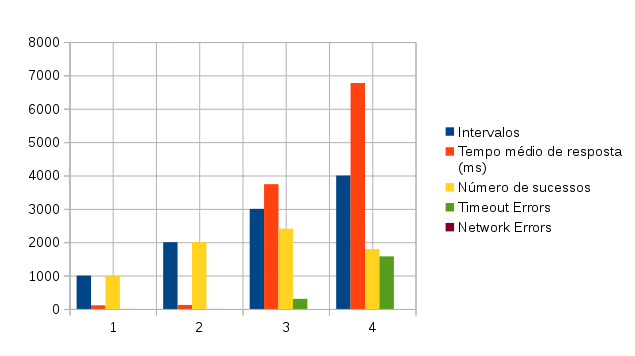
\includegraphics[width=.80\textwidth]{imagem/graficos/grafico_django_plano_de_teste_1.png}
    % Caption centralizada
    \captionsetup[grafico]{justification=centering}
    % Fonte
    \captionfont{\small{\textbf{\\Fonte: Autor}}}
  \end{grafico}
  
  Na interpretação do gráfico \ref{graf:teste-clientes-por-teste-django-a-1}  observa-se que apesar dos baixos números de sucessos o teste
  conseguiu alcançar até 4000 clientes, porém houve uma perda significativa no desempenho. 
  
  Entre 1000 a 2000 clientes por teste, acréscimo de 100\% do números de clientes, a aplicação se comportou bem respondendo as requisições com o tempo de resposta entre 
  107 a 118, ou seja um aumento pequeno de 10.67\%. O número de sucessos para 1000 clientes foi de 999.85 e para 2000 clientes foi de 1999.71, aumento
  de 100\% em relação ao número de clientes acrescidos. Nestes dois resultados houve poucos erros de tempo limite excedido. 
  
  Ao realizar o teste com 3000 clientes por teste, acréscimo de 100\% em relação ao teste anterior, houve um aumento significativo no tempo de resposta 
  que saltou de 118.42 milissegundos para 3737.71 milissegundos, aumento de  3056.31\% em relação ao teste anterior. A média do número de sucessos 
  teve um leve aumento saltando de 1999.71 para 2405.85, aumento de 20.30\%, caracterizando uma espera maior nas requisições e um baixo aumento
  de sucesso nas respostas destas requisiçoes. Um importante dado é a média de erros de tempo limite excedidos, que com o aumento de clientes,
  saltou de 0.28 para 301.14 de falhas de conexão à aplicação.
  
  No teste com 4000 clientes por teste, o tempo de resposta foi de 6771 milissegundos algo em torno de 6,76 segundos com  81.15\% de aumento
  em relação a 3000 clientes por teste. O número de sucessos caiu 25.49\% em relação aos dados do teste anterior chegando a ser menor que o
  teste com 2000 clientes por teste, com a média de 1999.71 contra 1792.57 com 4000 clientes. Houve também um alto índice de tempo limite excedido 
  neste plano de teste com um aumento de 1574.42\% para o teste com 3000 clientes. 
  
  Estes dados dos últimos dois teste, com 3000 e 4000 clientes caracteriza que a aplicação não suportou a alta escala de número de usuários infligida
  tendo um alto índice de espera nas requisições e também erros de tempo limite excedido. Ou seja o usuário não conseguiu nem conectar-se
  a API para buscar os dados do contato.
  
  Seguindo o mesmo modelo e conceitos de teste adotado para o protótipo Django, foi aplicado no plano de teste 
  B-1 correlacionado ao protótipo Node.Js. 
   
  \begin{table}[H]
    \centering
    \footnotesize
    % Alterar espaçamentos antes e depois do caption
    \setlength{\abovecaptionskip}{0pt}
    \setlength{\belowcaptionskip}{0pt}
    % Caption
    \caption[Teste B-1.1 com a API 1000 clientes]{Teste B 1.1 com a API Node.Js 1000 clientes}
    \label{tab:teste-b-1-1}
    % Conteúdo da tabela
    \begin{tabular}{c|c|c|c|c}
      \hline \hline
      Clientes  & 	Média de tempo de resposta (ms) \% &	Média do número de sucessos & 	Média de tempo limite excedido &	Média de erros de rede \\ 
      \hline \hline
      1000 &			12.57		 & 		1000	 		 & 		0 &					0 \\
      2000 (+100\%)&		12.42 (-1.19\%) & 		2000 (+100\%) & 			0 &					0 \\
      3000 (+100\%)&		12.14 (-2.25\%) & 		3000 (+100\%) & 			0 &					0 \\
      4000 (+100\%)&		12 (-1.15\%) & 			4000 (+100\%) & 			0 &					0 \\
      5000 (+100\%)&		12.42 (+3.49\%) & 		5000 (+100\%) & 			0 &					0 \\
      6000 (+100\%)&		12.42 (0\%) & 			6000 (+100\%) & 			0 &					0 \\
      7000 (+100\%)&		12.14 (-2.25\%) & 		7000 (+100\%) & 			0 &					0 \\
      8000 (+100\%)&		12.28 (+1.15\%) & 		7998.28 (+14.26\%) & 			0 &					0 \\
      9000 (+100\%)&		12.85 (+4.64\%) & 		9000 (+12.52\%) & 			0 &					0 \\
      10000 (+100\%)&		13.71 (+6.69\%) & 		9996.28 (+11.06\%)& 			0 &					0 \\
      \hline \hline
    \end{tabular}
    % Fonte
    \captionfont{\small{\textbf{\\Fonte: Autor}}}
  \end{table}
  
  A tabela \ref{tab:teste-b-1-1} mostra que a execução dos testes obteve a média de 12 milissegundos no tempo de resposta,
  respondendo em média as requisições corretamente de acordo com o número de sucessos, 0 na média de erros de tempo limite excedido 
  e 0 na média de erros de rede.
  
  Outro dado da tabela \ref{tab:teste-b-1-1} a ser salientado é que o plano de teste B-1 conseguiu alcançar o limite máximo suportado pela ferramenta
  Loader.io chegando aos 10000 clientes por testes. Aqui já podemos comprovar a eficiência do Node.Js em responder mais conexões com sucesso e suportar
  mais usuários que o protótipo Django. Sendo assim a série de teste ficou: B-1.1 com 1000 clientes, B-1.2 2000 clientes, 
  B-1.3 com 3000 clientes, B-1.4 com 4000 clientes, B-1.5 com 5000 clientes, B-1.6 com 6000 clientes, B-1.7 com 7000 clientes,
  B-1.8 com 8000 clientes, B-1.9 com 9000 clientes e B-1.10 com 10000 clientes.
  
  Comparando as duas tabelas \ref{tab:sumario-resultado-plano-teste-a-1} e \ref{tab:teste-b-1-1}, pode-se ver que 
  o tempo de resposta com o protótipo Node.Js fica em torno de 12 a 13 milissegundos ao contrário dos dados da tabela \ref{tab:sumario-resultado-plano-teste-a-1}
  
  Com os dados acima foi possível gerar o gráfico \ref{graf:teste-cliente-por-teste-node} referente aos testes 
  realizados com o Node.Js

  \begin{grafico}[H]
    % Alterar espaçamentos antes e depois do caption
    \setlength{\abovecaptionskip}{5pt}
    \setlength{\belowcaptionskip}{0pt}
    \label{graf:teste-cliente-por-teste-node}
    % Caption
    \caption[Cliente por teste Node.Js]
	    {Cliente por teste Node.Js}
    \centering
    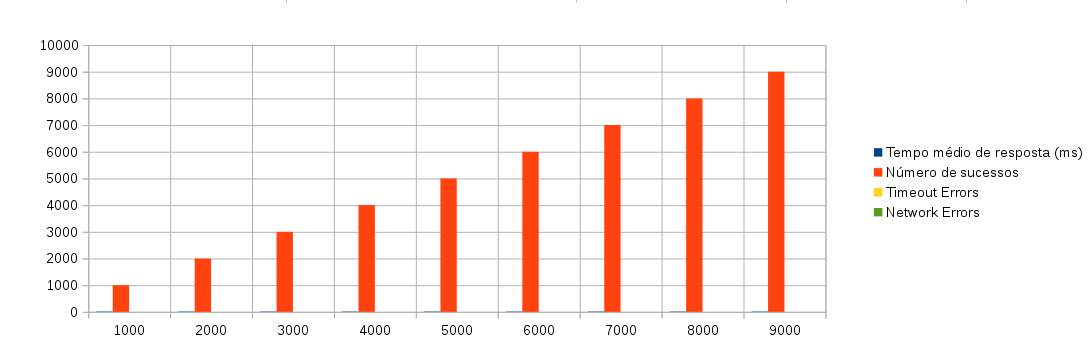
\includegraphics[width=.80\textwidth]{imagem/graficos/grafico_node_plano_de_teste_1.png}
    % Caption centralizada
    \captionsetup[grafico]{justification=centering}
    % Fonte
    \captionfont{\small{\textbf{\\Fonte: Autor}}}
  \end{grafico}
  
  Na interpretação do gráfico \ref{graf:teste-cliente-por-teste-node}  observa-se o tempo médio de resposta quase não se altera
  e o número de sucessos possui uma taxa de quase 100\% em relação ao número de clientes.
  
\subsection{Clientes por segundo}  
  
  Nesta seção é apresentado o plano de teste A-2 e B-2 que corresponde ao teste clientes por segundo da ferramenta loader.io. Irá
  ser realizado um sumário dos testes de cada protótipo e sua séries coletando as médias de cada execução.
  
  O teste será iniciado com 50 clientes conectando a API a cada segundo durante 1 minuto. Para cada série deste plano de teste
  será executado 7 vezes o mesmo teste e destes resultados será retirado a média dos tempos de resposta, média dos números de 
  sucessos, média dos erros de tempo de limite excedido e a média dos erros de rede. No decorrer de cada séria será acrescentado
  50 usuários até a quantidade máxima suportada pela aplicação.
  
  Veja o exemplo do teste A-2.1 o qual obteve os dados gerados pelo Loader.io.
  
  \begin{table}[H]
    \centering
    \footnotesize
    % Alterar espaçamentos antes e depois do caption
    \setlength{\abovecaptionskip}{0pt}
    \setlength{\belowcaptionskip}{0pt}
    % Caption
    \caption[Teste A-2.1 com a API Django 50 clientes]{Teste A 2.1 com a API Django 50 clientes}
    \label{tab:teste-a-2-1}
    % Conteúdo da tabela
    \begin{tabular}{c|c|c|c|c}
      \hline \hline
      Número de execução &	Tempo médio de resposta &	Número de sucessos &	Tempo limite excedido &	 Erros de rede \\
      \hline \hline
      Primeira execução &	1620 &				2500 &			0 &				0 \\
      Segunda execução &	1639 &				2269 &			0 &				0 \\
      Terceira execução &	1584 &				2359 &			0 &				0 \\
      Quarta execução  &	1627 &				2476 &			0 &				0 \\
      Quinta execução  &	1609 &				2563 &			0 &				0 \\
      Sexta execução   &	1560 &				2642 &			0 &				0 \\
      Sétima execução  &	1585 &				2579 &			0 &				0 \\
      Media & 			1603.42 &			2484 & 			0 &				0 \\
      \hline \hline
    \end{tabular}
    % Fonte
    \captionfont{\small{\textbf{\\Fonte: Autor}}}
  \end{table}
  
  A tabela \ref{tab:teste-a-2-1} mostra que na primeira execução do teste A-2.1 com 50 clientes conectando a aplicação por segundo
  durante 1 minuto de duração obteve-se 1620 milissegundos no tempo médio de resposta,
  2500 números de sucessos, 0 erros de tempo de limite, 0 erros de rede.
  
  Sendo assim o plano de teste A-2, realizou as séries A-3.1 com 50 clientes por segundo e A-2.2 com 100 clientes por segundo.
  Com os dados obtidos de cada teste pode-se fazer o sumário destes que serão apresentados 
  a seguir na tabela \ref{tab:sumario-resultado-plano-teste-a-2}.
  
  \begin{table}[H]
    \centering
    \footnotesize
    % Alterar espaçamentos antes e depois do caption
    \setlength{\abovecaptionskip}{0pt}
    \setlength{\belowcaptionskip}{0pt}
    % Caption
    \caption[Teste A-2 com a API Django]{Teste A-2 com a API Django}
    \label{tab:sumario-resultado-plano-teste-a-2}
    % Conteúdo da tabela
    \begin{tabular}{c|c|c|c|c}
      \hline \hline
      Clientes / segundo  & 	Média de tempo de resposta (ms) \% &	Média do número de sucessos & 	Média de tempo limite excedido &	Média de erros de rede \\ 
      \hline \hline
      50 &			1603,42 & 				2484 & 					0 &					0 \\
      100 (+100\%)&		4509,14 (+181.22\%) & 			1666,14 (-32.92\%) & 			200,85  &				0 \\
      \hline \hline
    \end{tabular}
    % Fonte
    \captionfont{\small{\textbf{\\Fonte: Autor}}}
  \end{table}
  
  A tabela \ref{tab:sumario-resultado-plano-teste-a-2} exibe as médias dos campos: média de tempo de resposta, 
  média do número de sucessos, média de erros de tempo de limite, média de erros de rede de cada teste executado 
  para o plano de teste A-2 do protótipo Django.
  
  Com os dados acima foi possível gerar o gráfico \ref{graf:teste-clientes-por-segundo-django} do 
  protótipo Django.
  
  \begin{grafico}[H]
    % Alterar espaçamentos antes e depois do caption
    \setlength{\abovecaptionskip}{5pt}
    \setlength{\belowcaptionskip}{0pt}
    
    % Caption
    \caption[Usuários por segundo no Django]
	    {Usuários por segundo no Django}
    \centering
    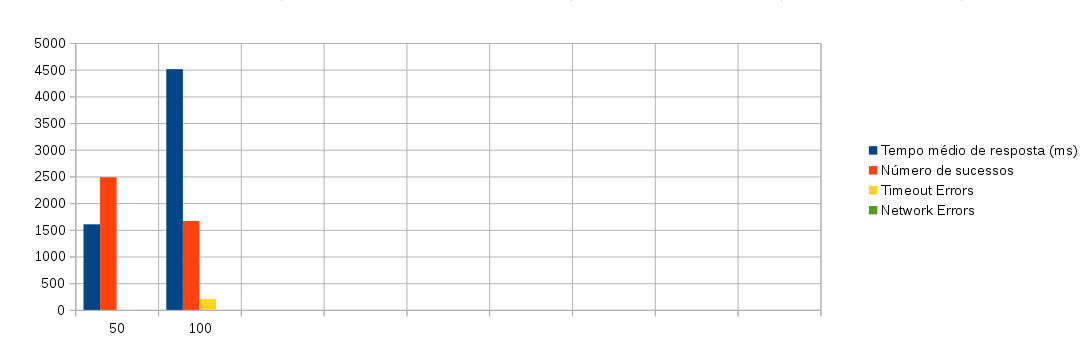
\includegraphics[width=.80\textwidth]{imagem/graficos/grafico_django_plano_de_teste_2.png}
    % Caption centralizada
    \captionsetup[grafico]{justification=centering}
    % Fonte
    \captionfont{\small{\textbf{\\Fonte: Autor}}}
    \label{graf:teste-clientes-por-segundo-django}
  \end{grafico}
  
  Ao interpretar o gráfico \ref{graf:teste-clientes-por-segundo-django}  observa-se que o máximo de clientes neste protótipo
  foi de apenas 100 clientes por segundo com uma taxa elevada na média do tempo de resposta 4509.14 ms. Taxa essa de 181.22\%
  em relação ao primeiro teste, inclusive a média de erros de tempo limite excedido aumento de zero para 200 erros . 
  Também é possível identificar que o número de sucessos teve uma queda de 32.92\% ficando apenas
  com a média de 1666.14 sucessos
 
  Seguindo o mesmo modelo e conceitos de teste adotado para o protótipo Django, foi aplicado no plano de teste 
  B-2 correlacionado ao protótipo Node.Js.
  
  \begin{table}[H]
    \centering
    \footnotesize
    % Alterar espaçamentos antes e depois do caption
    \setlength{\abovecaptionskip}{0pt}
    \setlength{\belowcaptionskip}{0pt}
    % Caption
    \caption[Teste B-2 com a API Node.Js]{Teste B-2 com a API Node.Js}
    \label{tab:teste-b-2}
    % Conteúdo da tabela
    \begin{tabular}{c|c|c|c|c}
      \hline \hline
      Clientes  & 	Média de tempo de resposta (ms) \% &	Média do número de sucessos & 	Média de tempo limite excedido &	Média de erros de rede \\ 
      \hline \hline
      50 &			12.85		 & 		3000 &					0 &					0 \\
      100 (+100\%)&		12.85 (0\%) & 			6000 (+100\%) & 			0 &					0 \\
      200 (+100\%)&		20.14 (+56.73\%) & 		11998.14 (+299.93\%) & 			0 &					0 \\
      300 (+100\%)&		311.42 (+1446.27\%) & 		17862 (+48.87\%) & 			5.28 &					0 \\
      400 (+100\%)&		1818.71 (+484.00\%) & 		16581.28 (-7.17\%) & 			119 (+2153.78) &			23.14 \\
      \hline \hline
    \end{tabular}
    % Fonte
    \captionfont{\small{\textbf{\\Fonte: Autor}}}
  \end{table}
  
  A tabela \ref{tab:teste-b-2} mostra que o protótipo consegue responder a uma escala de até 400 clientes por segunda
  porém com perdas nas conexões com o erro de tempo de limite excedido. Um ponto a observar que com a carga de 400 clientes por segundo 
  a média de tempo de resposta foi para 1.8 segundos diferente do outros testes em que a média do tempo de resposta ficava entre 12 e 14
  milissegundos.
  
  Continuando na tabela \ref{tab:teste-b-2} o plano de teste B-2 conseguiu 400 clientes por segundo, 300\% a mais que o teste 
  com o protótipo Django. A eficiência do Node.Js em responder mais conexões com sucesso e suportar
  mais usuários é bem melhor em relação ao protótipo Django. Sendo assim a série de teste ficou: B-2.1 com 50 clientes por segundo, 
  B-2.2 100 clientes por segundo,  B-2.3 com 200 clientes, B-2.4 com 300 clientes por segundo, B-2.5 com 400 clientes por segundo.
  
  Com os dados sumarizados foi possível gerar o gráfico \ref{graf:teste-cliente-por-segundo-node} referente aos testes 
  realizados com o Node.Js

  \begin{grafico}[H]
    % Alterar espaçamentos antes e depois do caption
    \setlength{\abovecaptionskip}{5pt}
    \setlength{\belowcaptionskip}{0pt}
    \label{graf:teste-cliente-por-segundo-node}
    % Caption
    \caption[Cliente por segundo Node.Js]
	    {Cliente por segundo Node.Js}
    \centering
    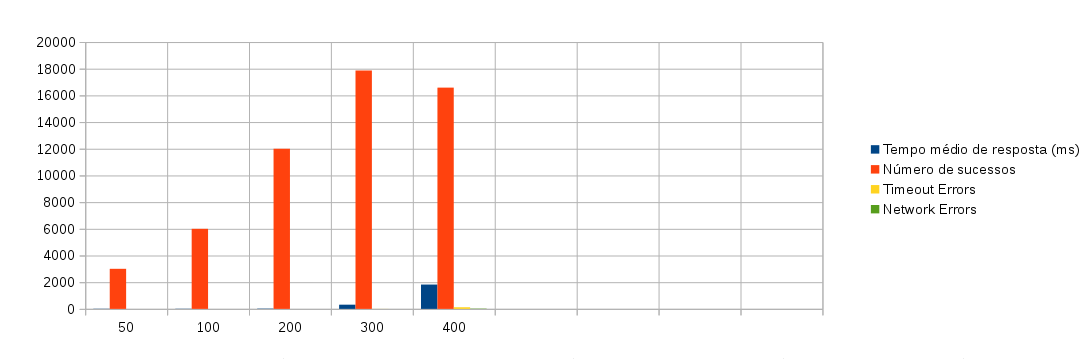
\includegraphics[width=.80\textwidth]{imagem/graficos/grafico_node_plano_de_teste_2.png}
    % Caption centralizada
    \captionsetup[grafico]{justification=centering}
    % Fonte
    \captionfont{\small{\textbf{\\Fonte: Autor}}}
  \end{grafico}
  
  Na interpretação do gráfico \ref{graf:teste-cliente-por-segundo-node} observa-se que a aplicação tem melhor desempenho
  com 300 clientes por segundo respondendo com sucesso a mais requisções que os outros testes. Neste gráfico não pode
  ser visto mas houve uma taxa muito pequena de erros de tempo limite excedido (5.28) como pode ser conferido na tabela
  \ref{tab:teste-b-2}.
  

    
\subsection{Manter a carga no Servidor}  

    
  Apresenta-se nesta seção o plano de teste A-3 e B-3 que corresponde ao teste manter carga de usuários no qual tem-se um sumário
  com as médias de cada execução.
  Para melhor instruir o leitor, esse teste inicia com 50 a 100 usuários conectados no sistema até 1 minuto de duração. Cada teste
  foi executado 7 vezes e destes resultados retiramos a média para o tempo de resposta, número de sucessos, erro de limite de tempo excedido
  e a média para erros de rede. No decorrer da série acrescentamos 50 usuários até a quantidade máxima suportada pela aplicação.
  
  Veja o exemplo do teste A-3.1 do qual obtivemos os dados gerados pela ferramenta:
  
  \begin{table}[H]
    \centering
    \footnotesize
    % Alterar espaçamentos antes e depois do caption
    \setlength{\abovecaptionskip}{0pt}
    \setlength{\belowcaptionskip}{0pt}
    % Caption
    \caption[Teste A-3.1 com a API Django 50 – 100 clientes]{Teste A 3.1 com a API Django 50 – 100 clientes}
    \label{tab:teste-a-3-1}
    % Conteúdo da tabela
    \begin{tabular}{c|c|c|c|c}
      \hline \hline
      Número de execução &	Tempo médio de resposta &	Número de sucessos &	Tempo limite excedido &	 Erros de rede \\
      \hline \hline
      Primeira execução &	1605 &				2754 &			0 &				0 \\
      Segunda execução &	1661 &				2659 &			0 &				0 \\
      Terceira execução &	1691 &				2610 &			0 &				0 \\
      Quarta execução  &	1678 &				2631 &			0 &				0 \\
      Quinta execução  &	1652 &				2674 &			0 &				0 \\
      Sexta execução   &	1634 &				2712 &			0 &				0 \\
      Sétima execução  &	1628 &				2707 &			0 &				0 \\
      Media & 			1649.85 &			2678.14 & 		0 &				0 \\
      \hline \hline
    \end{tabular}
    % Fonte
    \captionfont{\small{\textbf{\\Fonte: Autor}}}
  \end{table}
  
  A tabela \ref{tab:teste-a-3-1} mostra que na primeira execução do teste A-3.1 com o mínimo de 50 clientes até o máximo de 100 clientes
  durante 1 minuto de duração obteve-se 1605 milissegundos no tempo médio de resposta,
  2754 números de sucessos, 0 erros de tempo de limite, 0 erros de rede.
  
  Para este plano de teste A-3, foram realizados as séries A-3.1 de 50 a 100 clientes, A-3.2 de 100 a 150 clientes, A-3.3 de 150 a 200 clientes,
  A-3.4 de 200 a 250 clientes, A-3.5 de 250 a 300, A-3.6 de 300 e 350 clientes. Com os dados obtidos de cada teste pode-se fazer o sumário
  destes que serão apresentados a seguir na tabela \ref{tab:sumario-resultado-plano-teste-a-3}.
  
  \begin{table}[H]
    \centering
    \footnotesize
    % Alterar espaçamentos antes e depois do caption
    \setlength{\abovecaptionskip}{0pt}
    \setlength{\belowcaptionskip}{0pt}
    % Caption
    \caption[Sumário dos resultados do plano A-3]{Sumário dos resultados do plano A-3}
    \label{tab:sumario-resultado-plano-teste-a-3}
    % Conteúdo da tabela
    \begin{tabular}{c|c|c|c|c}
      \hline \hline
      Intervalos  & 	Média de tempo de resposta (ms) \% &	Número de sucessos & 	Erro de tempo de limite &	Erro de rede \\ 
      \hline \hline
      50 a 100 &		1649.85 &			2678.14 & 			0 &				0 \\
      100 a 150&		2663.14 (+61.41\%)&		2734.28 (+2.09\%)& 		2.85 (+2750\%) &		0 \\
      150 a 200&		5539.85 (+108.01\%)&		1487.42 (-45.60\%)& 		258.85 (+8982.45\%) &		0 \\
      200 a 250&		5452.28 (-1.58\%)&		1714.42 (+15.26\%)& 		574.42 (+121.91\%) &		0 \\
      250 a 300&		5964.14 (+9.38\%)&		1717.57 (+0.18\%)& 		810.57 (+41.11\%) &		0 \\
      300 a 350&		6256.71 (+4.90\%)&		1625.85 (-5.34\%)& 		935.28 (+15.38\%) &		0 \\
      \hline \hline
    \end{tabular}
    % Fonte
    \captionfont{\small{\textbf{\\Fonte: Autor}}}
  \end{table}
   
  A tabela \ref{tab:sumario-resultado-plano-teste-a-3} exibe as médias dos campos (média de tempo de resposta, 
  média do número de sucessos, média de erros de limite de tempo excedido e a média de erros de rede) de cada teste executado 
  para o plano de teste A-3 do protótipo Django.
  Com os dados acima foi possível gerar o gráfico \ref{graf:teste-mantendo-carga-usuario-django} do 
  protótipo Django.
  
  \begin{grafico}[H]
    % Alterar espaçamentos antes e depois do caption
    \setlength{\abovecaptionskip}{5pt}
    \setlength{\belowcaptionskip}{0pt}
    \label{graf:teste-mantendo-carga-usuario-django}
    % Caption
    \caption[Mantendo a carga de usuários no Django]
	    {Mantendo a carga de usuários no Django}
    \centering
    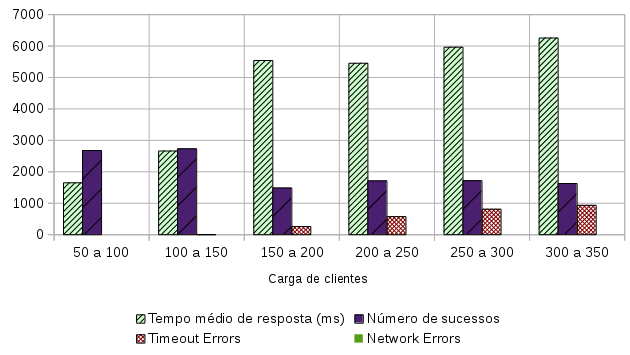
\includegraphics[width=.80\textwidth]{imagem/graficos/grafico_django_plano_de_teste_3.png}
    % Caption centralizada
    \captionsetup[grafico]{justification=centering}
    % Fonte
    \captionfont{\small{\textbf{\\Fonte: Autor}}}
  \end{grafico}
  
  Ao interpretar o gráfico \ref{graf:teste-mantendo-carga-usuario-django}  observa-se que com baixos números de clientes, no primeiro
  teste,o sistema teve a média de tempo de resposta(1649.85) para um alto número de sucessos (2678.14) . Ao elevar o número mínimo e máximo
  , no segundo teste, de clientes conectados observa-se que a média tempo de resposta foi quase a mesma da média de número de sucessos porém 
  a média do tempo de resposta teve um grande aumento, 61.41\% , em relação ao primeiro teste e o número de sucessos teve apenas 
  2.09\% de aumento.

  Com novos acréscimos de usuários no protótipo, elevando o número mínimo e máximo de clientes conectados, pode-se observar que o 
  tempo médio de resposta elevou-se em 108.01\% com 150 a 200 clientes comparando-o com o segundo teste que possui de 100 a 150 clientes.
  Com esta carga maior de usuários conectados o número de sucessos de cada requisição abaixou em comparação ao primeiro teste e segundo
  teste em 44.46\% e 45.60\% respectivamente. Concluindo que o protótipo já começa a dar indícios de perda de desempenho. Também é possível
  verificar, que a partir deste aumento de usuários houve a incidência de erros de tempo de limite excedido.
  
  Nas demais cargas realizadas o tempo médio de resposta teve uma ligeira queda, 1.58\% para o teste com 200 a 250 clientes, e nos dois
  últimos testes houve aumento no tempo de resposta. Vale lembrar que ha um aumento significativo na média de erro de tempo limite
  excedido de 261.32\% a partir de 150 a 200 clientes até 300 a 350 clientes.
  
  Este teste mostra que o protótipo Django possui pouca eficiência em lidar com usuários conectados ao sistema. Veja que os tempos de 
  resposta são altos e o número de sucessos são baixos para uma aplicação simples cujo objetivo é somente consumir as informações do banco de 
  dados através do método \textit{GET} da API.
  
  Seguindo o mesmo modelo e conceitos de teste adotado para o protótipo Django, foi aplicado no plano de teste 
  B-3 correlacionando ao protótipo Node.Js. 
  
  A partir do exemplo do teste B-3.1 o qual obtivemos os dados gerados pela ferramenta, já é possível comparar a eficiência das 
  tecnologias empregadas em cada protótipo.
  
  \begin{table}[H]
    \centering
    \footnotesize
    % Alterar espaçamentos antes e depois do caption
    \setlength{\abovecaptionskip}{0pt}
    \setlength{\belowcaptionskip}{0pt}
    % Caption
    \caption[Teste B-3.1 com a API Node.Js 50 – 100 clientes]{Teste B 3.1 com a API Node.Js 50 – 100 clientes}
    \label{tab:teste-b-3-1}
    % Conteúdo da tabela
    \begin{tabular}{c|c|c|c|c}
      \hline \hline
      Número de execução &	Tempo médio de resposta &	Número de sucessos &	Timeout Error &		 Network Errors \\
      \hline \hline
      Primeira execução &	229 &				19632 &			0 &				0 \\
      Segunda execução &	230 &				19514 &			0 &				0 \\
      Terceira execução &	233 &				19282 &			0 &				0 \\
      Quarta execução  &	230 &				19486 &			0 &				0 \\
      Quinta execução  &	235 &				19103 &			0 &				0 \\
      Sexta execução   &	231 &				19389 &			0 &				0 \\
      Sétima execução  &	240 &				18724 &			0 &				0 \\
      Media & 			232.57 &			19304.28 & 		0 &				0 \\
      \hline \hline
    \end{tabular}
    % Fonte
    \captionfont{\small{\textbf{\\Fonte: Autor}}}
  \end{table}
  
  A tabela \ref{tab:teste-b-3-1} mostra que a primeira execução do teste B-3.1, com o mínimo de 50 clientes até o máximo de 100 clientes
  durante 1 minuto de duração. Este teste obteve 232 milissegundos no tempo médio de resposta, valor muito inferior ao do plano de
  teste A-3.1 da tabela \ref{tab:teste-a-3-1} que foi de 1649.85 milissegundos, significando que a resposta para os usuários
  foi bem mais rápida do que o protótipo em Django. Vale ressaltar que o número de sucessos para cada conexão ficou em média de 
  19304.28, número superior ao teste A-3.1, de apenas 2754 números de sucessos.
  
  Outro dado importante a ser salientado é que no plano de teste B-3 conseguiu alcançar o limite de 450 a 500 usuários conectados
  na aplicação durante 1 minuto de duração. Valor este superior ao do plano de teste A-3 em que o limite de usuário chegou a apenas
  de 300 a 350 usuários conectados. Sendo assim a série de teste ficou B-3.1 de 50 a 100 clientes, B-3.2 de 100 a 150 clientes, 
  B-3.3 de 150 a 200 clientes, B-3.4 de 200 a 250 clientes, B-3.5 de 250 a 300, B-3.6 de 300 e 350 clientes, B-3.7 de 350 a 400 clientes,
  B-3.8 de 400 a 450 clientes, B-3.9 de 450 a 500 clientes. A partir deste número de clientes houve uma taxa de erro superior ao
  configurado na ferramenta. Com estes dados obtidos de cada teste pode-se fazer o sumário
  destes que serão apresentados a seguir na tabela \ref{tab:sumario-resultado-plano-teste-b-3}.
  
  \begin{table}[H]
    \centering
    \footnotesize
    % Alterar espaçamentos antes e depois do caption
    \setlength{\abovecaptionskip}{0pt}
    \setlength{\belowcaptionskip}{0pt}
    % Caption
    \caption[Sumário dos resultados do plano B-3]{Sumário dos resultados do plano B-3}
    \label{tab:sumario-resultado-plano-teste-b-3}
    % Conteúdo da tabela
    \begin{tabular}{c|c|c|c|c}
      \hline \hline
      Intervalos  & 	Média de tempo de resposta (ms) \% &	Número de sucessos & 	Erro de tempo de limite &	Erro de rede \\ 
      \hline \hline
      50 a 100 &		232.57  &			19304.28 &	 		0 &			0 \\
      100 a 150&		395 (+69.84\%)&			18964.14 (-1.76\%)&		0 &			0 \\
      150 a 200&		577 (+46.07\%)&			18125.71 (-4.42\%)& 		0 &			0 \\
      200 a 250&		764.28 (+32.45\%)&		17684.42 (-2.43\%)& 		0 &			0 \\
      250 a 300&		941.71 (+23.21\%)&		17471.85 (-1.20\%)& 		0 &			0 \\
      300 a 350&		1100.57 (+16.81\%)&		17655.42 (+1.05\%)& 		0 &			0 \\
      350 a 400&		1275.42 (+15.88\%)&		17406.85 (-1.40\%)& 		0 &			0 \\
      400 a 450&		1427 (+11.88\%)&		17675.42 (+1.54\%)& 		0 &			23.14 \\
      450 a 500&		1284.42 (-9.99\%)&		12579.57 (-28.83\%)& 		0 &			164.85 (+612.40\%)\\
      \hline \hline
    \end{tabular}
    % Fonte
    \captionfont{\small{\textbf{\\Fonte: Autor}}}
  \end{table}
   
  Assim como a tabela \ref{tab:sumario-resultado-plano-teste-a-3}, esta tabela \ref{tab:sumario-resultado-plano-teste-b-3} exibe as médias 
  dos campos (média de tempo de resposta, média do número de sucessos, média de erros de tempo de limite, média de erros de rede) 
  de cada teste executado para o plano de teste B-3 do protótipo Node.Js.
  
  Com os dados acima foi possível gerar o gráfico \ref{grafico:teste-mantendo-carga-usuario-node} referente aos testes 
  realizados com o Node.Js

  \begin{grafico}[H]
    % Alterar espaçamentos antes e depois do caption
    \setlength{\abovecaptionskip}{5pt}
    \setlength{\belowcaptionskip}{0pt}
    \label{grafico:teste-mantendo-carga-usuario-node}
    % Caption
    \caption[Mantendo a carga de usuários no Node.Js]
	    {Mantendo a carga de usuários no Node.Js}
    \centering
    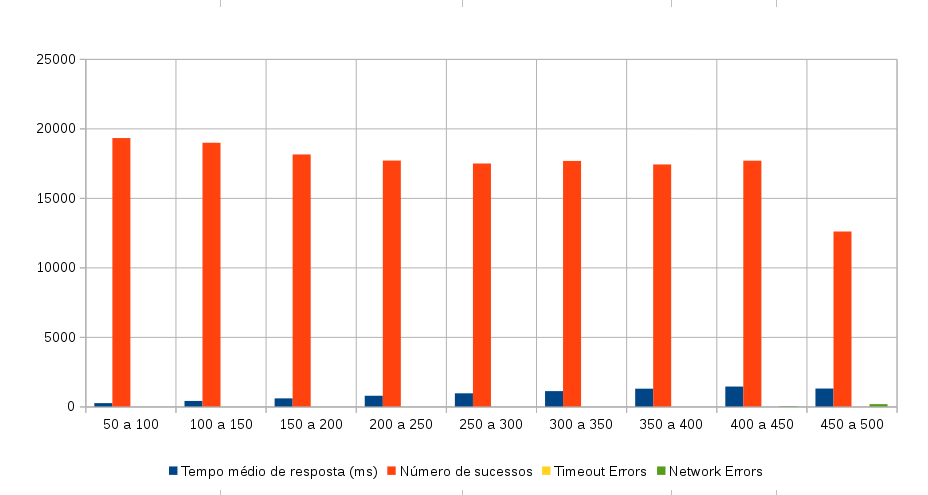
\includegraphics[width=.80\textwidth]{imagem/graficos/grafico_node_plano_de_teste_3.png}
    % Caption centralizada
    \captionsetup[grafico]{justification=centering}
    % Fonte
    \captionfont{\small{\textbf{\\Fonte: Autor}}}
  \end{grafico}

  No gráfico \ref{grafico:teste-mantendo-carga-usuario-node}  observa-se que o tempo de resposta das conexões 
  é muito baixo e o número de sucessos das conexões gira em torno de 17429 sucessos. Os valores da média de
  número de sucessos somente decrescem quando executa o teste de 450 a 500 usuários. Neste teste houve um alto número de erros 
  de rede o qual influenciou diretamente no número de sucessos.
  
  Neste mesmo gráfico pode-se ver que o número de erros de tempos de limite é sempre zero. Sendo assim podemos afirmar
  que não houve bloqueio nas operações de consulta a base de dados que poderiam impactar nos próximos testes.
  
  Comparando os dois gráficos \ref{grafico:teste-mantendo-carga-usuario-django} e \ref{grafico:teste-mantendo-carga-usuario-node} é
  visível a eficiência do protótipo em Node.Js pois em todos os campos o resultado obtido superou o primeiro protótipo.
  
  Pode-se concluir que o primeiro protótipo não tem condições de suportar grandes quantidades de usuários conectados ao
  sistema, visto o alto índice de erros de limite de tempo excedido, baixo número de sucessos e tempo de resposta alto, 
  conforme exposto na tabela \ref{tab:sumario-resultado-plano-teste-a-3}. Para o protótipo Django o número ideal de usuários
  conectados ao sistema fica em torno de 100 a 150 usuários enquanto em Node.Js tem-se 350 a 400 usuários conectados sem 
  erros.
  
  